\section{射影零点定理}\label{sec:projective-nullstellensatz}

如何把零点定理的叙述改成适用于射影情形的形式? 最直接的推广, 大概是希望对任意理想 $I\subseteq K[x_{0},\ldots,x_{n}]$ 都有
\begin{equation}\label{eq:naive-projective-nullstellensatz}
  \mathcal{I}_{\mathbb{P}}(\mathcal{V}_{\mathbb{P}}(I))=\sqrt{I}.
\end{equation}
然而, 这并不完全正确. 首先, 由于消没理想是齐次的, 我们或许应当只考虑齐次理想. 但即使在齐次理想中, 仍有一种情形使 \eqref{eq:naive-projective-nullstellensatz} 不成立:
\[
  I=\langle x_{0},\ldots,x_{n}\rangle.
\]
具体来说, 若 $I=\langle x_{0},\ldots,x_{n}\rangle$, 则 $\mathcal{V}_{\mathbb{P}}(I)$ 由使多项式 $x_{0},\ldots,x_{n}$ 全部消没的点 $[a_{0}:\cdots:a_{n}]\in\mathbb{P}^{n}$ 组成. 这只有在每个 $a_{i}=0$ 时才可能. 由于 $\mathbb{P}^{n}$ 中没有这样的点, 可知 $\mathcal{V}_{\mathbb{P}}(I)=\varnothing$. 每个多项式都空真地在 $\varnothing$ 的每一点处消没, 因而 $\mathcal{I}_{\mathbb{P}}(\mathcal{V}_{\mathbb{P}}(I))=K[x_{0},\ldots,x_{n}]$. 另一方面, 注意 $I=\langle x_{0},\ldots,x_{n}\rangle$ 是根理想 (事实上是极大理想), 故 $\sqrt{I}=\langle x_{0},\ldots,x_{n}\rangle$. 合并上述观察, 得
\[
  \mathcal{I}_{\mathbb{P}}(\mathcal{V}_{\mathbb{P}}(I))
    =K[x_{0},\ldots,x_{n}]\ne\langle x_{0},\ldots,x_{n}\rangle=\sqrt{I},
\]
这就给出了 \eqref{eq:naive-projective-nullstellensatz} 的一个反例. 为了避开 \eqref{eq:naive-projective-nullstellensatz} 的这一麻烦的例外, 我们给理想 $I=\langle x_{0},\ldots,x_{n}\rangle$ 取一个名字, 强调我们不愿考虑它.

\begin{Definition}{无关理想}\leavevmode\label{def:projective-irrelevant-ideal}
理想 $\langle x_{0},\ldots,x_{n}\rangle\subseteq K[x_{0},\ldots,x_{n}]$ 称为\emph{无关理想}. $K[x_{0},\ldots,x_{n}]$ 中不同于无关理想的理想称为\emph{相关理想}.
\end{Definition}

在下面射影零点定理的叙述中, 第一条断言是弱零点定理在射影情形下的自然对应, 第二条断言则是强零点定理的自然对应.

\begin{Theorem}{射影零点定理}\leavevmode\label{thm:projective-nullstellensatz}
设 $I\subseteq K[x_{0},\ldots,x_{n}]$ 为齐次理想.
\begin{enumerate}[label=\arabic*.]
  \item $\mathcal{V}_{\mathbb{P}}(I)=\varnothing$ 当且仅当 $\sqrt{I}\supseteq\langle x_{0},\ldots,x_{n}\rangle$.
  \item 若 $\sqrt{I}$ 相关, 则 $\mathcal{I}_{\mathbb{P}}(\mathcal{V}_{\mathbb{P}}(I))=\sqrt{I}$.
\end{enumerate}
\end{Theorem}

幸运的是, 射影零点定理可以从它的仿射版本推出, 不必重新发展所需的代数工具. 关键是暂且搁置前两节讨论的方法, 转而利用另一种在仿射几何和射影几何之间转换的方法: 仿射锥.

为了引出仿射锥的概念, 注意齐次理想有两种用法: 既可用它定义射影簇 $\mathcal{V}_{\mathbb{P}}(I)\subseteq\mathbb{P}^{n}$, 也可用它定义仿射簇 $\mathcal{V}_{\mathbb{A}}(I)\subseteq\mathbb{A}^{n+1}$. 先来看一个例子, 以了解这两种观点之间的关系.

\begin{Example}{$\mathcal{V}_{\mathbb{P}}(I)$ 与 $\mathcal{V}_{\mathbb{A}}(I)$ 的比较}\leavevmode\label{ex:projective-circle-and-affine-cone}
取 $K=\mathbb{R}$, 令 $I=\langle-x_{0}^{2}+x_{1}^{2}+x_{2}^{2}\rangle\subseteq\mathbb{R}[x_{0},x_{1},x_{2}]$. 则
\[
  \mathcal{V}_{\mathbb{P}}(I)
  =\{[a_{0}:a_{1}:a_{2}]\in\mathbb{P}^{2}\mid-a_{0}^{2}+a_{1}^{2}+a_{2}^{2}=0\}.
\]
若 $a_{0}\ne0$, 同比例缩放三个坐标便可假设 $a_{0}=1$. 另一方面, 若 $a_{0}=0$, 定义方程变成 $a_{1}^{2}+a_{2}^{2}=0$, 从而 $a_{1}=a_{2}=0$. 因为 $\mathbb{P}^{2}$ 中不存在 $a_{0}=a_{1}=a_{2}=0$ 的点, 所以
\[
  \mathcal{V}_{\mathbb{P}}(I)=\{[1:a_{1}:a_{2}]\in\mathbb{P}^{2}\mid-1+a_{1}^{2}+a_{2}^{2}=0\},
\]
它与 $\mathbb{A}^{2}$ 中的单位圆, 即仿射簇 $\mathcal{V}_{\mathbb{A}}(-1+x_{1}^{2}+x_{2}^{2})\subseteq\mathbb{A}^{2}$, 有自然双射.

\BookPairedFigure{
若改把 $I$ 看作定义 $\mathbb{A}^{3}$ 中的仿射簇, 则 $\mathcal{V}_{\mathbb{A}}(I)$ 是右图所示以原点为顶点的圆锥. (图中 $x_{0}$ 是竖直坐标.) 在图中可看到, 我们已等同于单位圆的射影簇 $\mathcal{V}_{\mathbb{P}}(I)$, 正是 $\mathcal{V}_{\mathbb{A}}(I)$ 与平面 $x_{0}=1$ 的交. 进一步注意, $\mathcal{V}_{\mathbb{A}}(I)$ 可以看作所有经过原点且在 Corollary~\ref{prop:projective-space-affine-plus-infinity} 的双射下对应于 $\mathcal{V}_{\mathbb{P}}(I)$ 中的点的直线的并.
}{
\phantomsection\label{fig:projective-cone-and-circle}%
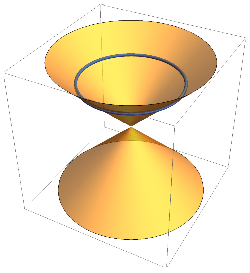
\includegraphics[width=\linewidth]{figures/projective-cone-and-circle.pdf}
}
\end{Example}

前一例中 $\mathcal{V}_{\mathbb{A}}(I)$ 是一个锥, 这并非巧合: 锥 $C\subseteq\mathbb{A}^{3}$ 具有如下性质, 只要 $(a_{0},a_{1},a_{2})\in C$, 那么整条直线
\[
  \{(\lambda a_{0},\lambda a_{1},\lambda a_{2})\mid\lambda\in K\}
\]
都包含在 $C$ 中. 从射影的观点看, 这就是说, 无论如何表示点 $[a_{0}:a_{1}:a_{2}]\in\mathbb{P}^{2}$, $[a_{0}:a_{1}:a_{2}]$ 是否属于 $C$ 都是良定义的. 有了 Example~\ref{ex:projective-circle-and-affine-cone} 的图像作为参照, 现在可以引入射影空间的子集上的仿射锥的精确定义.

\begin{Definition}{射影簇上的仿射锥}\leavevmode\label{def:affine-cone-over-projective-subset}
设 $X\subseteq\mathbb{P}^{n}$ 为一子集. $X$ 上的\emph{仿射锥}是集合
\[
  C(X)=\{(0,\ldots,0)\}\cup\{(a_{0},\ldots,a_{n})\mid[a_{0}:\cdots:a_{n}]\in X\}
  \subseteq\mathbb{A}^{n+1}.
\]
\end{Definition}

换句话说, 若 $X=\varnothing$, 则 $C(X)$ 只有原点; 否则, $C(X)$ 是与 $X\subseteq\mathbb{P}^{n}$ 中的点对应的所有过原点的直线的并. 例如, Example~\ref{ex:projective-circle-and-affine-cone} 中 $\mathcal{V}_{\mathbb{P}}(I)\subseteq\mathbb{P}^{2}$ 上的仿射锥等于 $\mathcal{V}_{\mathbb{A}}(I)\subseteq\mathbb{A}^{3}$. 这是下述引理的一个特例.

\begin{Lemma}{$\mathcal{V}_{\mathbb{A}}(I)=C(\mathcal{V}_{\mathbb{P}}(I))$}\leavevmode\label{lem:affine-vanishing-set-is-cone-of-projective-vanishing-set}
若 $I\subsetneq K[x_{0},\ldots,x_{n}]$ 为齐次理想, 则
\[
  \mathcal{V}_{\mathbb{A}}(I)=C\bigl(\mathcal{V}_{\mathbb{P}}(I)\bigr).
\]
\end{Lemma}
\begin{Proof}
首先注意, 对每个齐次理想 $I\subsetneq K[x_{0},\ldots,x_{n}]$, 有 $(0,\ldots,0)\in\mathcal{V}_{\mathbb{A}}(I)$. 为了看出这一点, 由 Proposition~\ref{prop:homogeneous-ideal-has-homogeneous-generators} 回顾, $I$ 有一组齐次生成元. 若 $(0,\ldots,0)\notin\mathcal{V}_{\mathbb{A}}(I)$, 则其中至少一个生成元必为满足 $f(0,\ldots,0)\ne0$ 的齐次多项式 $f$. 但不在 $(0,\ldots,0)$ 消没的齐次多项式只有非零常数多项式; 若 $I$ 的生成元中有这样的多项式, 则 $I=K[x_{0},\ldots,x_{n}]$, 与假设 $I\ne K[x_{0},\ldots,x_{n}]$ 矛盾.

因此, $(0,\ldots,0)\in\mathcal{V}_{\mathbb{A}}(I)$. 此外, 若 $(a_{0},\ldots,a_{n})$ 至少有一个非零坐标, 则 $I$ 的齐次性意味着
\[
  (a_{0},\ldots,a_{n})\in\mathcal{V}_{\mathbb{A}}(I)
  \iff[a_{0}:\cdots:a_{n}]\in\mathcal{V}_{\mathbb{P}}(I)
  \iff(a_{0},\ldots,a_{n})\in C(\mathcal{V}_{\mathbb{P}}(I)).
\]
这就证明了所断言的 $\mathcal{V}_{\mathbb{A}}(I)=C(\mathcal{V}_{\mathbb{P}}(I))$.
\end{Proof}

前一个引理用仿射锥联系了 $\mathcal{V}_{\mathbb{A}}$ 与 $\mathcal{V}_{\mathbb{P}}$ 算子, 下一个引理则用仿射锥联系 $\mathcal{I}_{\mathbb{A}}$ 与 $\mathcal{I}_{\mathbb{P}}$ 算子.

\begin{Lemma}{$\mathcal{I}_{\mathbb{P}}(X)=\mathcal{I}_{\mathbb{A}}(C(X))$}\leavevmode\label{lem:projective-ideal-equals-affine-ideal-of-cone}
若 $X\subseteq\mathbb{P}^{n}$ 为非空子集, 则
\[
  \mathcal{I}_{\mathbb{P}}(X)=\mathcal{I}_{\mathbb{A}}\bigl(C(X)\bigr).
\]
\end{Lemma}
\begin{Proof}
\BookPairedNote{
由于 $\mathcal{I}_{\mathbb{P}}(X)$ 是齐次理想, 它有一组齐次生成元. 由假设 $X\ne\varnothing$, 这些生成元都不可能是非零常数多项式. 因此它们全是正次数的齐次多项式, 从而在 $(0,\ldots,0)\in\mathbb{A}^{n+1}$ 处消没.
}{
Lemmas~\ref{lem:affine-vanishing-set-is-cone-of-projective-vanishing-set} 和~\ref{lem:projective-ideal-equals-affine-ideal-of-cone} 分别排除了 $I=K[x_{0},\ldots,x_{n}]$ 和 $X=\varnothing$. 这两项排除都是必要的; 见 Exercise~\ref{ex:necessity-of-affine-cone-lemma-hypotheses}.
}
所以, 对所有 $f\in\mathcal{I}_{\mathbb{P}}(X)$ 都有 $f(0,\ldots,0)=0$. 利用这一点, 可将 $\mathcal{I}_{\mathbb{P}}(X)$ 的定义重写如下:
\[
  \begin{aligned}
  \mathcal{I}_{\mathbb{P}}(X)
    &=\left\{f\in K[x_{0},\ldots,x_{n}]\ \middle|\
    \begin{gathered}
      \text{若 }[a_{0}:\cdots:a_{n}]\in X,\text{ 则 } f(a_{0},\ldots,a_{n})=0,\text{ 且}\\
      \text{若 }(a_{0},\ldots,a_{n})=(0,\ldots,0),\text{ 则 } f(a_{0},\ldots,a_{n})=0
    \end{gathered}\right\}\\
    &=\mathcal{I}_{\mathbb{A}}\bigl(\{(0,\ldots,0)\}\cup
      \{(a_{0},\ldots,a_{n})\mid[a_{0}:\cdots:a_{n}]\in X\}\bigr)\\
    &=\mathcal{I}_{\mathbb{A}}\bigl(C(X)\bigr),
  \end{aligned}
\]
如所断言.
\end{Proof}

有了 Lemmas~\ref{lem:affine-vanishing-set-is-cone-of-projective-vanishing-set} 和~\ref{lem:projective-ideal-equals-affine-ideal-of-cone}, 证明射影零点定理只需应用仿射零点定理.

\begingroup
\renewcommand{\AJProofBegin}{%
  \par\addvspace{\topsep}\noindent
  {\sffamily\bfseries\CJKfamily{pffont}Proof of Theorem~\ref{thm:projective-nullstellensatz}}\enspace\ignorespaces
}
\begin{Proof}
设 $I\subseteq K[x_{0},\ldots,x_{n}]$ 为齐次理想.

首先验证射影零点定理的第一条断言: $\sqrt{I}\supseteq\langle x_{0},\ldots,x_{n}\rangle$ 当且仅当 $\mathcal{V}_{\mathbb{P}}(I)=\varnothing$. 先假设 $\sqrt{I}\supseteq\langle x_{0},\ldots,x_{n}\rangle$. 那么
\[
  \mathcal{V}_{\mathbb{P}}(I)=\mathcal{V}_{\mathbb{P}}(\sqrt{I})
   \subseteq\mathcal{V}_{\mathbb{P}}(\langle x_{0},\ldots,x_{n}\rangle)=\varnothing,
\]
其中第一个等式就是 Exercise~\ref{ex:projective-vanishing-set-invariant-under-radical}. 反之, 假设 $\mathcal{V}_{\mathbb{P}}(I)=\varnothing$. 若 $I=K[x_{0},\ldots,x_{n}]$, 则 $\sqrt{I}=K[x_{0},\ldots,x_{n}]\supseteq\langle x_{0},\ldots,x_{n}\rangle$; 否则 $I\subsetneq K[x_{0},\ldots,x_{n}]$, 可用 Lemma~\ref{lem:affine-vanishing-set-is-cone-of-projective-vanishing-set} 得到
\[
  \mathcal{V}_{\mathbb{A}}(I)=C\bigl(\mathcal{V}_{\mathbb{P}}(I)\bigr)
    =C(\varnothing)=\{(0,\ldots,0)\},
\]
再由仿射零点定理得
\[
  \sqrt{I}=\mathcal{I}_{\mathbb{A}}(\mathcal{V}_{\mathbb{A}}(I))
  =\mathcal{I}_{\mathbb{A}}(\{(0,\ldots,0)\})=\langle x_{0},\ldots,x_{n}\rangle.
\]
两种情形都有 $\sqrt{I}\supseteq\langle x_{0},\ldots,x_{n}\rangle$, 这就证明了射影零点定理的第一部分.

为了证明射影零点定理的第二条断言, 假设 $\sqrt{I}$ 相关; 我们要证明 $\mathcal{I}_{\mathbb{P}}(\mathcal{V}_{\mathbb{P}}(I))=\sqrt{I}$. 先考虑 $\mathcal{V}_{\mathbb{P}}(I)=\varnothing$ 的情形. 由上述论证, $\sqrt{I}\supseteq\langle x_{0},\ldots,x_{n}\rangle$. 但包含 (极大的) 无关理想的相关理想只有整个环 $K[x_{0},\ldots,x_{n}]$, 故必有 $\sqrt{I}=K[x_{0},\ldots,x_{n}]$. 由于 $\mathcal{I}_{\mathbb{P}}(\mathcal{V}_{\mathbb{P}}(I))=\mathcal{I}_{\mathbb{P}}(\varnothing)=K[x_{0},\ldots,x_{n}]$, 断言 $\mathcal{I}_{\mathbb{P}}(\mathcal{V}_{\mathbb{P}}(I))=\sqrt{I}$ 在此情形下成立. 现在考虑 $\mathcal{V}_{\mathbb{P}}(I)\ne\varnothing$ 的情形. Lemma~\ref{lem:projective-ideal-equals-affine-ideal-of-cone} 给出
\[
  \mathcal{I}_{\mathbb{P}}(\mathcal{V}_{\mathbb{P}}(I))
    =\mathcal{I}_{\mathbb{A}}\bigl(C(\mathcal{V}_{\mathbb{P}}(I))\bigr).
\]
此外, 由于 $\mathcal{V}_{\mathbb{P}}(I)\ne\varnothing$, 必有 $I\subsetneq K[x_{0},\ldots,x_{n}]$, 故由 Lemma~\ref{lem:affine-vanishing-set-is-cone-of-projective-vanishing-set} 和仿射零点定理, 得
\[
  \mathcal{I}_{\mathbb{A}}\bigl(C(\mathcal{V}_{\mathbb{P}}(I))\bigr)
    =\mathcal{I}_{\mathbb{A}}(\mathcal{V}_{\mathbb{A}}(I))=\sqrt{I}.
\]
合并以上等式, 就得到了所需的 $\mathcal{I}_{\mathbb{P}}(\mathcal{V}_{\mathbb{P}}(I))=\sqrt{I}$.
\end{Proof}
\endgroup

和仿射情形一样, 射影零点定理的一个应用是显著简化射影消没理想的计算.

\begin{Example}{再看 $\mathbb{P}^{2}$ 中一条直线的消没理想}\leavevmode\label{ex:projective-line-ideal-by-nullstellensatz}
如 Example~\ref{ex:vanishing-ideal-of-projective-line-in-plane} 所示, 令 $X=\mathcal{V}_{\mathbb{P}}(x_{0}+x_{1}-x_{2})\subseteq\mathbb{P}^{2}$. 我们在 Exercise~\ref{ex:vanishing-ideal-of-projective-line-by-substitution} 中概述过直接计算 $\mathcal{I}_{\mathbb{P}}(X)$ 的方法. 有了射影零点定理, 现在只须注意 $\langle x_{0}+x_{1}-x_{2}\rangle$ 是消没集非空的齐次根理想. 因此
\[
  \mathcal{I}_{\mathbb{P}}(X)
  =\mathcal{I}_{\mathbb{P}}(\mathcal{V}_{\mathbb{P}}(\langle x_{0}+x_{1}-x_{2}\rangle))
  =\langle x_{0}+x_{1}-x_{2}\rangle.
\]
\end{Example}

与仿射情形完全相同, 射影零点定理也明确了射影 $\mathcal{V}$ 和 $\mathcal{I}$ 算子在哪些定义域上互逆. 于是可以给出射影簇与相应理想之间的下列对应表.

\begin{Proposition}{射影簇与理想}\leavevmode\label{prop:projective-variety-ideal-dictionary}
$\mathcal{V}_{\mathbb{P}}$ 和 $\mathcal{I}_{\mathbb{P}}$ 是互逆且反转包含关系的双射, 在下列理想和簇的层次之间建立对应:
\[
  \begin{array}{c@{\quad}c@{\quad}c}
  \left\{\begin{gathered}K[x_{0},\ldots,x_{n}]\text{ 中的}\\\text{相关齐次根理想}\end{gathered}\right\}
    &\longleftrightarrow&\{\mathbb{P}^{n}\text{ 中的射影簇}\}\\
  \rotatebox[origin=c]{90}{$\subseteq$} && \rotatebox[origin=c]{90}{$\subseteq$}\\
  \left\{\begin{gathered}K[x_{0},\ldots,x_{n}]\text{ 中的}\\\text{相关齐次素理想}\end{gathered}\right\}
    &\longleftrightarrow&\{\mathbb{P}^{n}\text{ 中的不可约簇}\}\\
  \rotatebox[origin=c]{90}{$\subseteq$} && \rotatebox[origin=c]{90}{$\subseteq$}\\
  \left\{\begin{gathered}K[x_{0},\ldots,x_{n}]\text{ 中的}\\\text{相关齐次极大理想}\end{gathered}\right\}
    &\longleftrightarrow&\{\mathbb{P}^{n}\text{ 中的点}\}.
  \end{array}
\]
\end{Proposition}
\begin{Proof}
设 $X\subseteq\mathbb{P}^{n}$ 为射影簇. 首先, 由 Proposition~\ref{prop:projective-vanishing-ideal-is-homogeneous-radical}, $\mathcal{I}_{\mathbb{P}}(X)$ 确实是 $K[x_{0},\ldots,x_{n}]$ 中的齐次根理想. 此外, $\mathcal{I}_{\mathbb{P}}(X)$ 不是无关理想. 为了说明这一点, 反设
\[
  \mathcal{I}_{\mathbb{P}}(X)=\langle x_{0},\ldots,x_{n}\rangle.
\]
于是 Proposition~\ref{prop:basic-properties-of-projective-vanishing-operators} 给出
\[
  X=\mathcal{V}_{\mathbb{P}}(\mathcal{I}_{\mathbb{P}}(X))
    =\mathcal{V}(\langle x_{0},\ldots,x_{n}\rangle)=\varnothing.
\]
但这样
\[
  \mathcal{I}_{\mathbb{P}}(X)=\mathcal{I}_{\mathbb{P}}(\varnothing)=K[x_{0},\ldots,x_{n}],
\]
与上述假设 $\mathcal{I}_{\mathbb{P}}(X)=\langle x_{0},\ldots,x_{n}\rangle$ 矛盾.

因此, $\mathcal{I}_{\mathbb{P}}$ 把 $\mathbb{P}^{n}$ 中任一射影簇映到 $K[x_{0},\ldots,x_{n}]$ 中的一个相关齐次根理想. 反过来, 按定义, $\mathcal{V}_{\mathbb{P}}$ 把任一这样的理想映到一个射影簇. 在这两个定义域上有
\[
  \mathcal{V}_{\mathbb{P}}(\mathcal{I}_{\mathbb{P}}(X))=X
  \qquad\text{和}\qquad
  \mathcal{I}_{\mathbb{P}}(\mathcal{V}_{\mathbb{P}}(I))=I,
\]
分别由 Proposition~\ref{prop:basic-properties-of-projective-vanishing-operators} 和射影零点定理得到. 这就证明了命题中的第一个双射. 余下两个双射由下列观察得出: $X$ 不可约当且仅当 $\mathcal{I}_{\mathbb{P}}(X)$ 为素理想 (Exercise~\ref{ex:projective-irreducibility-equivalent-to-prime-ideal}), 而 $X$ 是单个点当且仅当 $\mathcal{I}_{\mathbb{P}}(X)$ 是极大理想 (Exercise~\ref{ex:projective-single-point-equivalent-to-maximal-ideal}).
\end{Proof}

本章开始培养对射影簇的直观认识, 并以射影情形下的零点定理告一段落. 现在我们已经熟悉射影簇, 下一项任务是引入并研究它们之间保持结构的映射. 下一章将讨论这一主题.

\BookExerciseHeading
\begin{BookExercises}
  \item\label{ex:real-affine-cone-over-projective-conic} 在实数域上画出射影簇
  \[
    X=\mathcal{V}_{\mathbb{P}}(x^{2}-yz)\subseteq\mathbb{P}^{2}
  \]
  上的仿射锥. (计算机绘图软件或许有帮助.) 在图上的什么位置能看到仿射限制
  \[
    X_{0}=\mathcal{V}_{\mathbb{A}}(x^{2}-y)\subseteq\mathbb{A}^{2}?
  \]
  \item\label{ex:necessity-of-affine-cone-lemma-hypotheses}
  \begin{enumerate}
    \item 说明若 $I=K[x_{0},\ldots,x_{n}]$, Lemma~\ref{lem:affine-vanishing-set-is-cone-of-projective-vanishing-set} 不成立.
    \item 说明若 $X=\varnothing$, Lemma~\ref{lem:projective-ideal-equals-affine-ideal-of-cone} 不成立.
  \end{enumerate}
  \item\label{ex:projective-vanishing-set-invariant-under-radical} 设 $I\subseteq K[x_{0},\ldots,x_{n}]$ 为理想. 证明
  \[
    \mathcal{V}_{\mathbb{P}}(I)=\mathcal{V}_{\mathbb{P}}(\sqrt I).
  \]
  \item\label{ex:projective-vanishing-ideal-of-irreducible-polynomial} 设 $f\in K[x_{0},\ldots,x_{n}]$ 是不可约齐次多项式, 令 $X=\mathcal{V}_{\mathbb{P}}(f)\subseteq\mathbb{P}^{n}$. 证明 $\mathcal{I}_{\mathbb{P}}(X)=\langle f\rangle$.
  \item\label{ex:projective-vanishing-ideal-via-distinct-irreducible-factors} 设 $f\in K[x_{0},\ldots,x_{n}]$ 是非常数齐次多项式, 令 $X=\mathcal{V}_{\mathbb{P}}(f)\subseteq\mathbb{P}^{n}$. 用 $f$ 的互异不可约因子描述 $\mathcal{I}_{\mathbb{P}}(X)$.
  \item\label{ex:empty-projective-variety-criterion-by-degree} 证明 $\mathcal{V}_{\mathbb{P}}(f_{1},\ldots,f_{k})=\varnothing$ 当且仅当存在非负整数 $d$, 使每个 $d$ 次单项式均属于 $\langle f_{1},\ldots,f_{k}\rangle$.
\end{BookExercises}
